LF \cite{lf,logicalframeworks} is a logical framework, i.e., a formal language that we use to define other formal languages. It is a very advanced language, so advanced that we were only able to understand it in the 1980s. Therefore, it is very hard to learn and should only be attempted after gaining a solid basis of knowledge about logic. On the other hand, the intuitions underlying LF are strikingly simple and the precise definition of LF is actually quite short.

The major problem with learning LF is that LF goes together with a certain methodology of approaching logics. This methodology is so powerful and elegant that users of LF become very familiar with it, so much that they forget there is any other way to do it. Consequently, they often apply this methodology even when describing LF itself, thus scaring everybody off who has not embraced it yet. That makes it virtually impossible to learn LF on your own.

Therefore, we will go a different route here: We will ignore the foundations of LF altogether and focus on how we can use LF in practice. \emph{The goal is to show that LF is simple, natural, and practical rather than -- as many are inadvertently led to think -- difficult, weird, and esoteric.}

\section{The Context-Free Fragment}

\begin{quote}
 Lesson 1: LF is just a tool that we use to write down grammars. For convenience, we give the productions names.
\end{quote}

\paragraph{Grammars and Named Productions}
Consider the grammar of propositional logic over a fixed set $\Sigma$ of propositional variables:

\begin{center}
\begin{tabular}{lcl@{\tb}l}
$\FORM$ & $::=$ & $\true$ & \emph{truth} \\
     &  $|$  & $\false$ & \emph{falsity} \\
     &  $|$  & $\FORM \wedge \FORM$ & \emph{conjunction} \\
     &  $|$  & $\FORM \vee \FORM$ & \emph{disjunction} \\
     &  $|$  & $\FORM \impl \FORM$ & \emph{implication} \\
     &  $|$  & $\neg \FORM$ & \emph{negation} \\
     &  $|$  & $p$ where $p\in\Sigma$ & \emph{boolean variables}\\
\end{tabular}
\end{center}

Moreover, assume $p,q\in\Sigma$ and consider this example of a syntax tree for the formula $(\true\wedge p) \vee q$:

\begin{center}
\begin{tikzpicture}
\node (0) at (0,0) {$\FORM$};
\node (01) at (-1,-1) {$\FORM$};
\node (02) at (1,-1) {$\FORM$};
\node (011) at (-2,-2) {$\FORM$};
\node (012) at (0,-2) {$\FORM$};
\node (011') at (-2,-3) {$\true$};
\node (02') at (1,-2) {$q$};
\node (012') at (0,-3) {$p$};
\begin{scope}[gray]
\node (01t') at (-1,-2) {$\wedge$};
\node (0t') at (0,-1) {$\vee$};
\draw[dashed] (0) -- (0t');
\draw[dashed] (01) -- (01t');
\end{scope}
\draw[-\arrowtip] (0) -- (01);
\draw[-\arrowtip] (0) -- (02);
\draw[-\arrowtip] (01) -- (011);
\draw[-\arrowtip] (01) -- (012);
\draw[-\arrowtip] (02) -- (02');
\draw[-\arrowtip] (011) -- (011');
\draw[-\arrowtip] (012) -- (012');
\end{tikzpicture}
\end{center}

As usual, every node corresponds to a subformula of $(\true\wedge p) \vee q$ and is labelled with the non-terminal symbol with which the derivation of that subformula begins. In particular, the root corresponds to the whole formula and every leaf node to an atomic formula. Moreover, some nodes produce additional terminal symbols (given in gray).

The key property of a syntax tree is that every node is connected to its children via a production. With a tiny change, we are able to state that much more elegantly: We give the productions names.

Giving names to production is very natural, for example, we can use

\begin{center}
\begin{tabular}{lcl@{\tb}l}
$\FORM$ & $::=$ & $\rulename{truth} \rnsep \true$ & \\
     &  $|$  & $\rulename{falsity} \rnsep\false$ &  \\
     &  $|$  & $\rulename{conj} \rnsep \FORM \wedge \FORM$ &  \\
     &  $|$  & $\rulename{disj} \rnsep \FORM \vee \FORM$ &  \\
     &  $|$  & $\rulename{impl} \rnsep \FORM \impl \FORM$ &  \\
     &  $|$  & $\rulename{neg} \rnsep \neg \FORM$ & \\
     &  $|$  & $V_p \rnsep p$ where $p\in\Sigma$ \\
\end{tabular}
\end{center}

Note that naming the productions actually helps documenting and reading the grammar.

Now that the productions have names, we can use them to label the nodes in the syntax tree:

\begin{center}
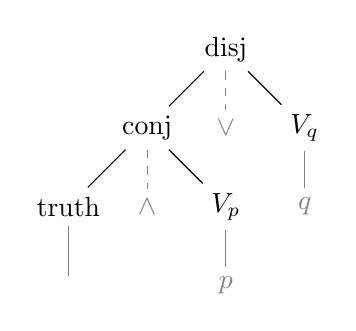
\begin{tikzpicture}
\node (0) at (0,0) {\rlname{disj}};
\node (01) at (-1,-1) {\rlname{conj}};
\node (02) at (1,-1) {$V_q$};
\node (011) at (-2,-2) {\rlname{truth}};
\node (012) at (0,-2) {$V_p$};
\begin{scope}[gray]
\node (01t') at (-1,-2) {$\wedge$};
\node (0t') at (0,-1) {$\vee$};
\node (011') at (-2,-3) {$\true$};
\node (02') at (1,-2) {$q$};
\node (012') at (0,-3) {$p$};
\draw[-\arrowtip] (02) -- (02');
\draw[-\arrowtip] (011) -- (011');
\draw[-\arrowtip] (012) -- (012');
\draw[dashed] (0) -- (0t');
\draw[dashed] (01) -- (01t');
\end{scope}
\draw[-\arrowtip] (0) -- (01);
\draw[-\arrowtip] (0) -- (02);
\draw[-\arrowtip] (01) -- (011);
\draw[-\arrowtip] (01) -- (012);
\end{tikzpicture}
\end{center}

Now we observe that the nodes for the terminal symbols are actually redundant. Indeed, if productions have names, we do not need terminal symbols (given in gray above) \emph{in a syntax tree}. Just like brackets, the sole purpose of $\wedge$ and $\vee$ is as a visual aid to display formulas nicely \emph{in a line}. And the terminal symbols like $\true$, $p$, and $q$ are redundant because they are determined by the name of the preceding production.

There is no commonly used convention how to write named productions in BNF. For example, we use an ad-hoc notation and write our grammar as follows:

\begin{center}
\begin{tabular}{lcl@{\tb}l}
$\FORM$ & $::=$ & $\rlname{truth} \rnsep $ & \\
     &  $|$  & $\rlname{falsity} \rnsep $ &  \\
     &  $|$  & $\rlname{conj} \rnsep \FORM, \FORM$ &  \\
     &  $|$  & $\rlname{disj} \rnsep \FORM, \FORM$ &  \\
     &  $|$  & $\rlname{impl} \rnsep \FORM, \FORM$ &  \\
     &  $|$  & $\rlname{neg} \rnsep \FORM$ & \\
     &  $|$  & $V_p \rnsep $ where $p\in\Sigma$ \\
\end{tabular}
\end{center}

This may look a bit unusual, but observe that it still contains the same information as our original grammar.

\paragraph{Grammars in LF}
Grammars with named productions can be written down in LF directly. The basic idea is that non-terminal symbols and (named) productions are introduced by one declaration each:
\begin{enumerate}
\item For a non-terminal symbol $A$, we write $\idecl{A}{\type}$.
\item For a production $A::=\rnsep A_1\;\ldots A_n$, we write $\idecl{P}{A_1\arr\ldots\arr A_n\arr A}$.
\end{enumerate}

Our grammar becomes
\begin{twelfsig}
\decl{\FORM}{\type} \\
\decl{\rlname{truth}}{\FORM}\\
\decl{\rlname{falsity}}{\FORM}\\
\decl{\rlname{conj}}{\FORM\arr\FORM\arr\FORM}\\
\decl{\rlname{disj}}{\FORM\arr\FORM\arr\FORM}\\
\decl{\rlname{impl}}{\FORM\arr\FORM\arr\FORM}\\
\decl{\rlname{neg}}{\FORM\arr\FORM}\\
\decl[$\mfor p\in\Sigma$]{V_p}{\FORM}\\
\end{twelfsig}
In LF text files, $\arr$ is written as $-\!\!>$.

One might argue that the notation with $\type$ and $\arr$ is somewhat arbitrary and even weird. Indeed, other notations can be more intuitive. Just for comparison, this is how the same grammar is written in SML:
\begin{lstlisting}[mathescape]
datatype $\FORM$ =
   $\rlname{truth}$
 | $\rlname{falsity}$
 | $\rlname{conj}$    of $\FORM$ * $\FORM$
 | $\rlname{disj}$    of $\FORM$ * $\FORM$
 | $\rlname{impl}$    of $\FORM$ * $\FORM$
 | $\rlname{neg}$    of $\FORM$ * $\FORM$
 | $\rlname{V_p}$                           for $p$ in $\Sigma$
\end{lstlisting}
Note how there is one \lstinline|datatype| for each non-terminal and one constructor for each production.

The specific notation of LF is in fact chosen very carefully and is very intuitive. But we will understand why only after learning a lot more about type theory.

\paragraph{Syntax Trees in LF}
In LF, we cannot only write down grammars but also syntax trees.
Our example tree from above is written in LF as
 \[(\rlname{conj}\;(\rlname{disj}\;\rlname{truth}\; V_p)\;V_q).\]
We only need brackets and whitespace to make sure that this linear representation can be uniquely translated back into a syntax tree.

This way of writing trees goes back to Lisp's S-expressions. It's also how SML does it. Some people might prefer the equivalent
\[\rlname{conj}(\rlname{disj}(\rlname{truth},V_p),V_q).\]

If we want to use XML, we can write a syntax tree like in OpenMath:
\begin{lstlisting}
<OMA>
  <OMS name="conj"/>
  <OMA><OMS name="disj"/><OMS name="truth"/><OMS name="V_p"/></OMA>
  <OMS name="V_q"/>
</OMA>
\end{lstlisting}

The bottom line is: We're now able to talk about syntax trees as objects! Instead of having to treat formulas as strings, we can treat them as syntax trees.

\section{The Context-Sensitive Fragment}\label{sec:lffe:cs}

\begin{quote}
 Lesson 2: It's useful to have productions that recurse into expressions with holes. LF supports that elegantly.
\end{quote}

Let's first understand what we mean by ``expressions with holes''.

\subsection{Expressions with Holes}\label{sec:lffe:holes}

\paragraph{Leaving Holes}
Consider our grammar for first-order logic:
\begin{center}
\begin{tabular}{lcl@{\tb}l}
$\FORM$ & $::=$ & $\true$ & \emph{truth} \\
        &  $|$  & $\false$ & \emph{falsity} \\
        &  $|$  & $\FORM \wedge \FORM$ & \emph{conjunction} \\
        &  $|$  & $\FORM \vee \FORM$ & \emph{disjunction} \\
        &  $|$  & $\FORM \arr \FORM$ & \emph{implication} \\
        &  $|$  & $\neg \FORM$ & \emph{negation} \\
        &  $|$  & $\forall \VAR\; \FORM$ & \emph{universal quantification} \\
        &  $|$  & $\exists \VAR\; \FORM$ & \emph{existential quantification} \\
        &  $|$  & $\TERM \doteq \TERM$ & \emph{equality} \\
        &  $|$  & $p(\overbrace{\TERM,\ldots,\TERM}^n)$ where $p\in\Sigma_p$ and $\arit(p)=n$& \emph{atomic formulas} \\
$\TERM$ & $::=$ & $f(\overbrace{\TERM,\ldots,\TERM}^n)$ where $f\in\Sigma_f$ and $\arit(f)=n$ & \emph{constants and function terms} \\
        &  $|$  & $\VAR$ & \emph{variables} \\
$\VAR$  & $::=$ & some countable set of names & \emph{variable names}
\end{tabular}
\end{center}

There is something fishy about this grammar, namely the non-terminal $\VAR$ with its vague production. This happens because -- contrary to propositional logic -- first-order logic is a language with binding, e.g., the $x$ is bound in $\forall x\;F$.
\medskip

Just like the named productions above, we can obtain a more elegant treatment of binding with a small conceptual leap: We introduce expressions with holes.

For example, let $F$ be the formula $f(x,y)\doteq g(y)$. $F$ has two variables -- $x$ and $y$ -- which we think of as placeholders for arbitrary terms. Let's make the placeholders explicit in the syntax tree:

\begin{center}
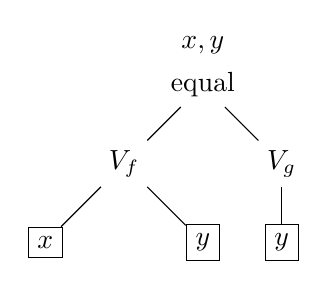
\begin{tikzpicture}
\node (H) at (0,.5) {$x,y$};
\node (0) at (0,0) {\rlname{equal}};
\node (01) at (-1,-1) {$V_f$};
\node (02) at (1,-1) {$V_g$};
\node[draw,rectangle] (011) at (-2,-2) {$x$};
\node[draw,rectangle] (012) at (0,-2) {$y$};
\node[draw,rectangle] (021) at (1,-2) {$y$};
\draw[-\arrowtip] (0) -- (01);
\draw[-\arrowtip] (0) -- (02);
\draw[-\arrowtip] (01) -- (011);
\draw[-\arrowtip] (01) -- (012);
\draw[-\arrowtip] (02) -- (021);
\end{tikzpicture}
\end{center}

The placeholder nodes are boxed to indicate that they do not represent productions but unknown subtrees that will be determined later.
To emphasize the holes in an expression, we will always list them above the root of the syntax tree.

\paragraph{Filling Holes}
Holes are placeholders for unknown expressions. Once known, we can plug in any expression for such a place holder. For example, in the expression $F$ above, we can plug the syntax tree for $f(c)$ into the hole $y$:

\begin{center}
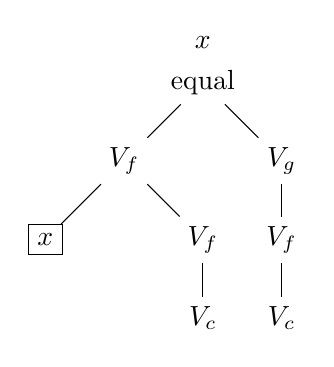
\begin{tikzpicture}
\node (H) at (0,.5) {$x$};
\node (0) at (0,0) {\rlname{equal}};
\node (01) at (-1,-1) {$V_f$};
\node (02) at (1,-1) {$V_g$};
\node[draw,rectangle] (011) at (-2,-2) {$x$};
\node (012) at (0,-2) {$V_f$};
\node (021) at (1,-2) {$V_f$};
\draw[-\arrowtip] (0) -- (01);
\draw[-\arrowtip] (0) -- (02);
\draw[-\arrowtip] (01) -- (011);
\draw[-\arrowtip] (01) -- (012);
\draw[-\arrowtip] (02) -- (021);
\node (0121) at (0,-3) {$V_c$};
\node (0211) at (1,-3) {$V_c$};
\draw[-\arrowtip] (012) -- (0121);
\draw[-\arrowtip] (021) -- (0211);
\end{tikzpicture}
\end{center}

Note that it is important that the holes are named: If a hole is used multiple times, we must plug in the same subtree everywhere. Also note that the resulting syntax tree only has one hole $x$.
\medskip

\paragraph{Expressions with Holes in General}
Of course, plugging in expressions for holes is exactly what we know already from first-order logic as the substitution of expressions for free variables. But note that we can use expressions with named holes \emph{for any grammar}. For example, let $G$ be the expression $a \impl (b \wedge a)$ of propositional logic with two holes $a$ and $b$; its syntax tree is

\begin{center}
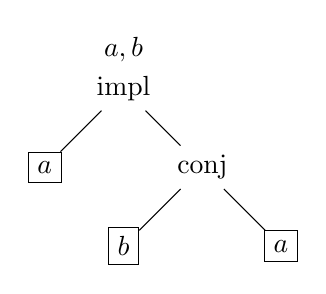
\begin{tikzpicture}
\node (H) at (0,.5) {$a,b$};
\node (0) at (0,0) {\rlname{impl}};
\node[draw,rectangle] (01) at (-1,-1) {$a$};
\node (02) at (1,-1) {\rlname{conj}};
\node[draw,rectangle] (021) at (0,-2) {$b$};
\node[draw,rectangle] (022) at (2,-2) {$a$};
\draw[-\arrowtip] (0) -- (01);
\draw[-\arrowtip] (0) -- (02);
\draw[-\arrowtip] (02) -- (021);
\draw[-\arrowtip] (02) -- (022);
\end{tikzpicture}
\end{center}

Note that we cannot generally plug in any subtree for any placeholder. For example, in $F$ above, we can only plug in terms for $x$ and $y$, i.e., a subtree whose root production is for the non-terminal $\TERM$. We call $\TERM$ the \emph{type} of the placeholders $x$ and $y$.

Let $H$ be the expression, $(f(x,y)\doteq g(y))\wedge a$; it has three holes, two of type $\TERM$ and one of type $\FORM$. Let's make the types explicit in our notation for syntax trees and write:

\begin{center}
\begin{tikzpicture}
\node (H) at (1,1.5) {$x:\TERM,y:\TERM,a:\FORM$};
\node (R) at (1,1) {\rlname{conj}};
\node[draw,rectangle] (R1) at (2,0) {$a$};
\node (0) at (0,0) {\rlname{equal}};
\node (01) at (-1,-1) {\rlname{V_f}};
\node (02) at (1,-1) {$V_g$};
\node[draw,rectangle] (011) at (-2,-2) {$x$};
\node[draw,rectangle] (012) at (0,-2) {$y$};
\node[draw,rectangle] (021) at (1,-2) {$y$};
\draw[-\arrowtip] (R) -- (0);
\draw[-\arrowtip] (R) -- (R1);
\draw[-\arrowtip] (0) -- (01);
\draw[-\arrowtip] (0) -- (02);
\draw[-\arrowtip] (01) -- (011);
\draw[-\arrowtip] (01) -- (012);
\draw[-\arrowtip] (02) -- (021);
\end{tikzpicture}
\end{center}

In this case, the types of the placeholders are redundant because the grammar forces us to plug in a term for $x$ and $y$ and a formula for $a$. It is still good to mark the types in the grammar: Firstly, it avoids confusion; secondly, the types are not always redundant.


\paragraph{Writing Expressions with Holes in LF}
LF lets us write expressions with holes explicitly. $G$ from above is written as
\[[a][b] (\rlname{impl}\;a\;(\rlname{\wedge}\;b\;a).\]
In LF, the holes of an expressions are always made explicit by prefixing the expressions with $[h]$ for every hole named $h$.

Again, we can argue about the notation. Some people prefer writing $G(a,b)$ or sometimes $G[a,b]$ if they want to emphasize that $G$ has two holes $a$ and $b$.

LF also lets us plug expressions into holes. If we want to plug in $\true$ for $a$ and $\false$ for $b$ in $G$, we write simply $G\;\true\;\false$. The result is the expression
\[G\;\true\;\false \;=\;\rlname{impl}\;\true\;(\rlname{\wedge}\;\false\;\true)\]
without holes.

Again, some people prefer the notation $G(\true,\false)$; that is incidental. The bottom line is: We can write expressions with holes easily and concisely in LF.
\medskip

LF also lets us make the types of placeholders explicit if we want to. For example, $H$ from above is written with explicit types as
\[[x:\TERM][y:\TERM][a:\FORM](\rlname{conj}\;(\rlname{equal}\;(V_f\;x\;y)\;y)\;a)\]

\subsection{Expressions with Holes as Operations}\label{sec:lffe:defs}

Every expression $E$ with a hole $x$ can be seen as an operation: The input is some other expressions $E'$; the output is the result of plugging $E'$ into the hole $E$. We can think of $E$ as a program, $E'$ as the input, and substitution as the machine that executes the program.

Since LF does substitution for us, we can directly use substitution to introduce some abbreviations. Consider the expression \[[a:\FORM][b:\FORM](\rlname{conj}\;(\rlname{impl}\;a\;b)\;(\rlname{impl}\;b\;a)),\]

In LF, we can introduce a name for any expression, with or without holes. If we want to call the expression above \rlname{equiv}, we write
\[\idecl{\rlname{equiv}}{\FORM\arr\FORM\arr\FORM \;=\;[a:\FORM][b:\FORM](\rlname{conj}\;(\rlname{impl}\;a\;b)\;(\rlname{impl}\;b\;a))}.\]

We can now write
 \[\rlname{equiv}\;\rlname{true}\;\rlname{false}\]
and substitution yields
  \[\rlname{equiv}\;\rlname{true}\;\rlname{false}\;=\;\rlname{conj}\;(\rlname{impl}\;\rlname{true}\;\rlname{false})\;(\rlname{impl}\;\rlname{false}\;\rlname{true})\]


\subsection{Productions using Expressions with Holes}

We've seen already that holes in expressions are nothing special. We usually call them \emph{free variables}, and they work in every grammar.

Using this intuition, we can now understand binding as an operation on expressions with holes.\footnote{This idea is called \emph{higher-order abstract syntax}. It is one of the most important ideas in the area of logical frameworks and a central principle of LF.} For example, we can understand the universal quantifier $\forall$ as an operator that takes a single argument: a formula with a hole of type $\TERM$.
\medskip

Again the BNF notation for grammars does not provide a notation for productions that use expressions with holes. Therefore, we have to introduce one ourselves again. Consider two non-terminals $A$ and $B$. Just like $B$ represents the collection of all expressions derived from $B$, we write $\{x:A\}B$ for the collection of all expressions derived from $B$ that have a hole named $x$ of type $A$.

For example, consider the production
 \[\FORM::=\rlname{conj}\rnsep\FORM\wedge\FORM.\]
We can read it as
\begin{center}
  ``The production \rlname{conj} takes two $\FORM$s and produces a $\FORM$.''
\end{center}
Similarly, we read the new production
 \[\FORM::=\rlname{univ}\rnsep\,\{x:\TERM\}\FORM\]
as
\begin{center}``The production \rlname{univ} takes a $\FORM$ with a hole $x$ for a $\TERM$ and produces a $\FORM$.''\end{center}
\medskip

With named productions and expressions with holes, our grammar for first-order logic becomes
\begin{center}
\begin{tabular}{lcl@{\tb}l}
$\FORM$ & $::=$
               & $\rlname{truth}\rnsep$ & \\
     &  $|$  & $\rlname{falsity}\rnsep$ &  \\
     &  $|$  & $\rlname{conj}\rnsep\FORM, \FORM$ &  \\
     &  $|$  & $\rlname{disj}\rnsep\FORM, \FORM$ &  \\
     &  $|$  & $\rlname{impl}\rnsep\FORM, \FORM$ &  \\
     &  $|$  & $\rlname{neg}\rnsep \FORM$ & \\
     &  $|$  & $\rlname{univ}\rnsep \{x:\TERM\} \FORM$ & \\
     &  $|$  & $\rlname{exist}\rnsep \{x:\TERM\} \FORM$ & \\
     &  $|$  & $\rlname{equal}\rnsep\TERM, \TERM$ &  \\
     &  $|$  & $V_p\rnsep\overbrace{\TERM,\ldots,\TERM}^n$ where $p\in\Sigma_p$ and $\arit(p)=n$& \\
$\TERM$ & $::=$ & $V_f\rnsep\overbrace{\TERM,\ldots,\TERM}^n$ where $f\in\Sigma_f$ and $\arit(f)=n$ & \\
        &  $|$  & $x$ & \\
\end{tabular}
\end{center}

For example, let $K$ be the formula $\forall x\;(p(x) \wedge \exists y\;q(u,y,v))$. Its syntax tree is

\begin{center}
\begin{tikzpicture}
\tikzstyle{bvar}=[dashed,rectangle,draw]
\tikzstyle{fvar}=[rectangle,draw]
\tikzstyle{level 3}=[sibling distance=3cm]
\tikzstyle{level 4}=[sibling distance=2cm]
\tikzstyle{edge from parent}+=[-\arrowtip]
\node at (0,.5) {$u:\TERM,v:\TERM$};
\path[level distance=1.3cm]
 node at (0,0) {\rlname{univ}}
  child {node {\rlname{conj}}
    child {node {$V_p$}
      child {node[bvar] {$x$}}
    }
	  child {node {\rlname{exist}}
	    child {node {$V_q$}
	      child {node[fvar] {$u$}}
        child {node[bvar] {$y$}}
        child {node[fvar] {$v$}}
        edge from parent node[right] {$y:\TERM$}
      }
    }
    edge from parent node[right] {$x:\TERM$}
  };
\end{tikzpicture}
\end{center}

Note how the nodes labelled with the productions $\rlname{univ}$ and $\rlname{exist}$ are followed by subtrees with holes. As before, the name of the hole is given above the respective subtree. Note that $x$ and $y$ are not holes of the overall tree; we say that they are \emph{bound}. To distinguish them from holes of the whole tree, we use dashed boxes for the bound holes.

%This grammar is not equivalent to the above grammar for first-order logic -- it is better. The above grammar permitted any formula as the argument to the universal quantification. Our new grammars permits exactly the terms with one hole.

\paragraph{Productions with Holes in LF}
We can write down our new grammar for first-order logic directly in LF:

\begin{twelfsig}
\decl{\FORM}{\type} \\
\decl{\TERM}{\type} \\
\decl{\rlname{truth}}{\FORM}\\
\decl{\rlname{falsity}}{\FORM}\\
\decl{\rlname{conj}}{\FORM\arr\FORM\arr\FORM}\\
\decl{\rlname{disj}}{\FORM\arr\FORM\arr\FORM}\\
\decl{\rlname{impl}}{\FORM\arr\FORM\arr\FORM}\\
\decl{\rlname{neg}}{\FORM\arr\FORM}\\
\decl{\rlname{equal}}{\TERM\arr\TERM\arr\FORM}\\
\decl{\rlname{univ}}{(\{x:\TERM\}\FORM)\arr\FORM}\\
\decl{\rlname{exist}}{(\{x:\TERM\}\FORM)\arr\FORM}\\
\decl[where $p\in\Sigma_p$ and $\arit(p)=n$]{V_p}{\overbrace{\TERM\arr\ldots\arr\TERM}^n\arr\;\FORM}  \\
\decl[where $f\in\Sigma_f$ and $\arit(f)=n$]{V_f}{\overbrace{\TERM\arr\ldots\arr\TERM}^n\arr\;\TERM} \\
\end{twelfsig}

%LF forces us to write $\{\_:\TERM\}\FORM$ instead of simply $\{\TERM\}\FORM$. There is a reason for that, and we will come back to it later.

The LF notation for syntax trees over these grammars is straightforward. For example, the formula $K$ is written in LF as 
\[[u:\TERM][v:\TERM]\;\rlname{univ}\;([x:\TERM]\;\rlname{conj}\;(p\;x)\;(\rlname{exist}\;([y:\TERM]\;V_q\;u\;y\;v)))\]
or -- if we omit the types of the placeholders -- as
\[[u][v]\;\rlname{univ}\;([x]\;\rlname{conj}\;(p\;x)\;(\rlname{exist}\;([y]\;V_q\;u\;y\;v)))\]

\section{Notation Declarations}

It is awkward to write syntax trees as
\[[u][v]\;\rlname{univ}\;([x]\;\rlname{conj}\;(p\;x)\;(\rlname{exist}\;([y]\;V_q\;u\;y\;v)))\]
because they are quite different from the nice notation
\[\forall x\;(p(x) \wedge \exists y\;q(u,y,v))\]
that we are used to. We can use a couple of syntactic sugars to tweak the LF notation into looking nicer.

\paragraph{Nice Identifiers}
We can give the productions any names we want. Most of the time, we can use the corresponding terminal symbol as the rule name. Moreover, we can use Unicode characters in identifiers. So we can change our grammar to

\begin{twelfsig}
\decl{\FORM}{\type} \\
\decl{\TERM}{\type} \\
\decl{\true}{\FORM}\\
\decl{\false}{\FORM}\\
\decl{\wedge}{\FORM\arr\FORM\arr\FORM}\\
\decl{\vee}{\FORM\arr\FORM\arr\FORM}\\
\decl{\impl}{\FORM\arr\FORM\arr\FORM}\\
\decl{\neg}{\FORM\arr\FORM}\\
\decldefnl{\equiv}{\FORM\arr\FORM\arr\FORM}{[a:\FORM][b:\FORM](\wedge\;(\impl\;a\;b)\;(\impl\;b\;a))} \\
\decl{\doteq}{\TERM\arr\TERM\arr\FORM}\\
\decl{\forall}{(\{x:\TERM\}\FORM)\arr\FORM}\\
\decl{\exists}{(\{x:\TERM\}\FORM)\arr\FORM}\\
\decl[where $p\in\Sigma_p$ and $\arit(p)=n$]{p}{\overbrace{\TERM\arr\ldots\arr\TERM}^n\arr\;\FORM}  \\
\decl[where $f\in\Sigma_f$ and $\arit(f)=n$]{f}{\overbrace{\TERM\arr\ldots\arr\TERM}^n\arr\;\TERM} \\
\end{twelfsig}
Note that we include the abbreviation for equivalence from Sect.~\ref{sec:lffe:defs}.

and now our example formula is written as
\[[u][v]\;\forall\;([x]\;\wedge\;(p\;x)\;\exists\;([y]\;q\;u\;y\;v)))\]

\paragraph{Notations}
We can also give notations to identifiers.
A notation consists of
\begin{itemize}
 \item fixity: prefix, infix (only for binary operators), or postfix
 \item if the fixity is infix, associativity: left, right, or none \\
   The associativity determines whether $P\;a\;Q\;a\;R$ is parsed as $(P\;a\;Q)\;a\;R$ (left), parsed as $P\;a\;(Q\;a\;R)$ (right), or forbidden (none).
   \footnote{Note that there is no such thing as an associative operator in LF.}
 \item precedence: a positive integer\\
  Higher precedences bind stronger, which permits omitting brackets.
\end{itemize}

We should make $\wedge$, $\vee$, $\impl$, $\equiv$, and $\doteq$ infix, and $\neg$ prefix.
$\wedge$ and $\vee$ should be left- or right-associative so that we can write $P\wedge Q\wedge R$. $\impl$ and $\equiv$ should have no associativity to avoid ambiguity.
$\neg$ should have a higher precedence than the other operators so that the brackets in $P\wedge (\neg Q)$ can be omitted. Finally, $\doteq$ should have a high precedence so that the brackets in $P\wedge (s\doteq t)$ can be omitted.

We can achieve that by adding the following notations to our grammar:

\begin{lstlisting}
%infix left 10 $\wedge$.
%infix left 10 $\vee$.
%infix none 10 $\impl$.
%infix none 10 $\equiv$.
%prefix 15 $\neg$.
%infix none 20 $\doteq$.
\end{lstlisting}

Then our example expression becomes:
\[[u][v]\;\forall\;([x]\;(p\;x)\wedge\exists\;([y]\;q\;u\;y\;v)))\]

Finally, LF uses the convention that the $[-]$ operator has the lowest possible precedence. Therefore, brackets around $([x]F)$ can often be omitted.
Our example expression finally becomes:
\[[u][v]\;\forall\;[x]\;(p\;x)\wedge\exists\;[y]\;(q\;u\;y\;v)\]

Note that this looks almost as nice as $\forall x\;(p(x) \wedge \exists y\;q(u,y,v))$. But the former is a syntax tree that we can work with directly whereas the latter is a string!


\section{The Fragment with Unary Dependent Types}

\begin{quote}
Lesson 3: It's often useful to have infinite families of non-terminals. LF supports that elegantly.
\end{quote}

Let's first understand why we would like to have infinitely many non-terminals.

\subsection{Families of Non-Terminals}

\paragraph{Proofs as Expressions}
So far we have seen how we can use LF to concisely write down context-sensitive grammars and expressions with holes. The main strength of LF is that we have a canonical linear notation for syntax trees of expressions.

In the area of logic, there is another kind of tree structure that is dominant: proofs. We have already seen how proofs can be represented as tree whose nodes are labelled with inference rules. Now we observe: This is basically the same principle as having syntax trees whose nodes are labelled with productions.

A production governs how we form new expressions from existing ones. Similarly, an inference rule governs how we form new proofs from existing ones. If we just think of them as syntax trees and productions, both of them become the same thing!

{\renewcommand{\der}{}
Compare a production, e.g., \rlname{impl}
\[\FORM::=\rlname{impl} \rnsep \FORM,\FORM\]
with an inference rule, e.g., modus ponens
\[\ibnc{\der F\impl G}{\der F}{\der G}{mp}\]
They look different, but that's just because we use very different notations. We see that if we write both of them as inference rules
\[
\ibnc{\FORM}{\FORM}{\FORM}{\rlname{impl}}
\tb\tb
\ibnc{\der F\impl G}{\der F}{\der G}{mp}
\]
or both of them as productions
\[
\FORM::=\rlname{impl} \rnsep \FORM,\FORM
\tb\tb
\der G \;::=\; mp \rnsep \der F\impl G, \;\der F
\]

\paragraph{Formulas as Non-Terminals}
However, there is one subtlety: In the case of inference rules, we do not have a finite set of non-terminal symbols. Indeed, the left side of the ``production'' for $mp$ is $\der G$ where $G$ is an arbitrary formula. Everything would work if we had a way of getting a fresh non-terminal symbol for every formula. But because we have infinitely many formulas, this is not possible right away.

Therefore, LF makes a third (after named productions and expressions with holes) key addition to our understanding of grammars: infinite families of non-terminal symbols. More concretely, if $A:\type$ is a non-terminal symbol, then we may add an $A$-indexed family $B$ of non-terminal symbols as $B:A\arr\type$.
}

For example, we introduce a $\FORM$-indexed family $\PROOF$ of non-terminal symbols as \[\PROOF:\FORM\arr\type.\] Then we have for every formula $F$ a non-terminal symbol $\PROOF\; F$. Expressions derived from $\PROOF\; F$ are the proofs of $F$.

Now we can in fact write our inference rule $mp$ like this
\[
\PROOF\; G \;::=\; mp \rnsep \PROOF\;(F\impl G), \;\PROOF\; F
\]

\subsection{Dependent Type Constructors in LF}

We have already seen the LF syntax for families of non-terminals above. For propositional logic, we declare our non-terminals as

\begin{twelfsig}
\decl{\FORM}{\type} \\
\decl{\PROOF}{\FORM\arr\type} \\
\end{twelfsig}

We can think of $\PROOF$ as an operator that takes one argument and returns a non-terminal symbol. Then ordinary non-terminals like $\FORM$ are the special case of non-terminals with $0$ arguments. In LF, we call the non-terminals \emph{types}. Non-terminals like $\PROOF\;F$ are called \emph{dependent types} because they depend on an expression.

The productions for $\FORM$ stay the same. And we want to write the production for $mp$ as 
\[\mathll{
\text{``$mp$ takes a proof of $F\impl G$ and a proof of $F$ and produces a proof of $G$.''}\nl[.5cm]
\ibnc{\der F\impl G}{\der F}{\der G}{mp}\nl[.5cm]
\idecl{mp}{\PROOF\;(F\impl G)\arr\PROOF\;F\arr\PROOF\;G}
}\]
\medskip

But there is still a small problem: In all three of the above formulations of the rule, $F$ and $G$ occur out of nowhere. We kind of know that they are intended to be arbitrary formulas, but we're not precise about it. Therefore, let's say
\begin{center}
``$mp$ takes a formula $F$, a formula $G$, a proof of $F\impl G$, and a proof of $F$\\ and produces a proof of $G$.''
\end{center}
Now we notice something special that was hidden by the notation before: $mp$ is a production that takes $4$ arguments, but \emph{the value of the first two arguments determines the type of the last two and of the return type}. This has become possible because of dependent types, and it is the most characteristic feature of dependent type theory.
\medskip

Therefore, we finally write $mp$ in LF as a production with two placeholders:
\[mp \;:\; \{F:\FORM\}\{G:\FORM\}\,\PROOF\;(F\impl G)\arr\PROOF\;F\arr\PROOF\;G\]
\medskip

Then our grammar for propositional logic looks like this:

\begin{twelfsig}
\decl{\FORM}{\type} \\
\decl{\PROOF}{\FORM\arr\type} \\[.5cm]
\decl{\rlname{truth}}{\FORM}\\
\decl{\rlname{falsity}}{\FORM}\\
\decl{\rlname{conj}}{\FORM\arr\FORM\arr\FORM}\\
\decl{\rlname{disj}}{\FORM\arr\FORM\arr\FORM}\\
\decl{\rlname{impl}}{\FORM\arr\FORM\arr\FORM}\\
\decl{\rlname{neg}}{\FORM\arr\FORM}\\
\decl[$\mfor p\in\Sigma$]{V_p}{\FORM}\\[.5cm]
\decl{mp}{\{F:\FORM\}\{G:\FORM\}\,\PROOF\;(F\impl G)\arr\PROOF\;F\arr\PROOF\;G} \\
\decl{\wedge E_l}{\{F:\FORM\}\{G:\FORM\}\,\PROOF\;(F\wedge G)\arr\PROOF\;F}\\
\decl{\wedge E_r}{\{F:\FORM\}\{G:\FORM\}\,\PROOF\;(F\wedge G)\arr\PROOF\;G}\\
\decl{\wedge I}{\{F:\FORM\}\{G:\FORM\}\,\PROOF\;F\arr\PROOF\;G\arr\PROOF\;(F\wedge G)} \\
\end{twelfsig}

Here we have already included the rules for conjunction:
\[\ianc{F\wedge G}{F}{\wedge E_l} \tb\tb \ianc{F\wedge G}{G}{\wedge E_r} \tb\tb \ibnc{F}{G}{F\wedge G}{\wedge I}\]

Of course, we're still missing all the other proof rules.
We could write them down already as well, but it's better to make the LF background a tiny bit more formal first using Sect.~\ref{sec:lffe:types}.
\medskip

Moreover, we can now declare axioms: An axiom asserting the formula $F$ is declared as a symbol that returns a proof of $F$. That makes sense because axioms are like additional proofs that exist a priori.

For example, consider the theory of semigroups is the first-order signature with a binary function symbol and an axiom for associativity. We obtain it by adding declarations to first-order logic, one for the function and one for the axiom:

\begin{twelfsig}
\tsig{Semigroup}\\
\decl[{\infix[$\circ$]{left}{30}}]{\circ}{\TERM\arr\TERM\arr\TERM}\\
\decl{\rlname{assoc}}{\PROOF\;\big(\forall [x] \forall[y]\forall[z] (x\circ y)\circ z \doteq x \circ (y\circ z)\big)} \\
\tsigend
\end{twelfsig}

Here we make use of an additional feature of Twelf: We can give a list of declarations a name using the keywork \lfkw{sig}.

Note that we give $\circ$ a higher precedence than $\doteq$ to save brackets.

\section{A Little More Background}\label{sec:lffe:types}

\subsection{Non-Terminals = Types}

The basic idea behind the formal syntax of LF is that we have two sorts of objects: expressions and types. \emph{Expressions} (sometimes also called \emph{terms}) represent syntax and proof trees. \emph{Types} classify the expressions; in particular, every non-terminal is a type. Every expression has exactly one type, and for an expression $E$ of type $T$, we write $E:T:\type$.

Thus, in order to understand the syntax of LF, we should understand what expressions and types there are. Let us review the different LF constructions that we have seen so far.

\begin{enumerate}
 \item Plain expressions representing syntax/proof trees. Their type is given by the non-terminal from which they are derived. E.g.,
   \[(\true\vee p)\wedge q\;:\;\FORM\;:\;\type.\]
 \item Expressions with holes
   \begin{itemize}
     \item Expressions with one hole. Their type is the form $\{x:A\}B$ where $A$ is the type of the hole $x$ and $B$ is the type of the whole expression. E.g.,
   \[[x:\TERM](x\;\doteq\;x)\;:\;\{x:\TERM\}\FORM\;:\;\type\]
  Note that a $[-]$-expression always has the corresponding $\{-\}$-type.
     \item Expressions with multiple holes are a special case: They are formed by chaining the above construction. E.g.,
   \[[x:\TERM][a:\FORM](x\;\doteq\;x)\wedge a\;:\;\{x:\TERM\}\{a:\FORM\}\FORM\;:\;\type\]
     \item Individual productions are expressions themselves. Their type is given in their declaration.
        E.g., $\neg:\FORM\arr\FORM$ is one of our productions, and we obtain
        \[\neg\;:\;\FORM\arr\FORM\;:\;\type\]
        When we write down LF formally, this becomes just a special case of an expression with a hole: Indeed, we \emph{define} $\FORM\arr\FORM$ as an abbreviation of $\{a:\FORM\}\FORM$ (for some arbitrary name $a$), and we employ the \emph{axiom}\footnote{This is called $\eta$-conversion.}
        \[\neg \; = \; [a:\FORM]\neg a\]
        That makes sense because $\neg$ and $[a:\FORM]\neg a$ behave in the same way according to $(\ast)$ below, namely
        \[\neg\;F \;=\; ([a:\FORM]\neg a)\;F.\]
   \end{itemize}
 \item Expressions formed by application
    \begin{itemize}
      \item Expressions formed by applying a production to another expression. Their type arises by removing one argument type. E.g., $\neg:\FORM\arr\FORM$ is a production that takes one argument of type $\FORM$, and if we apply it to another formula, we obtain
   \[\neg\;((\true\vee p)\wedge q)\;:\;\FORM\;:\;\type\]
      \item Expressions formed by applying a production to multiple expressions are a special case: They are formed by chaining the above construction, e.g.,
   \[\begin{array}{lclcl}
      mp & : & \{F:\FORM\}\{G:\FORM\}\,\PROOF\;(F\impl G)\arr \PROOF\;F\arr\PROOF\;G & : & \type\\
      mp\;\true & : & \{G:\FORM\}\,\PROOF\;(\true\impl G)\arr \PROOF\;\true\arr\PROOF\;G & : & \type\\
      mp\;\true\;p & : & \PROOF\;(\true\impl p)\arr \PROOF\;\true\arr\PROOF\;p & : & \type\\
    \end{array}\]
    and so on.
    \item Expressions formed by plugging an expression into a hole are a special case of application as well. Indeed, we have
    \[[a:\FORM]\neg a\;:\;\{a:\FORM\}\FORM\;:\;\type,\] and thus
    \[([a:\FORM]\neg a)\;F\;:\;\FORM\;:\;\type\]
    for any formula $F$. Note that we already know the result of plugging $F$ into the hole $a$, namely $\neg\;F$. Therefore, we employ the \emph{axiom}\footnote{This is called $\beta$-conversion.}
    \[([a:\FORM]\neg a)\;F \;=\;\neg\;F. \tb\tb(\ast)\]
  \end{itemize}
\end{enumerate}

\noindent
Note that we only need four basic constructions to form all the LF expressions:
\begin{enumerate}
 \item constants are atomic and must have been introduced by declarations; we distinguish the declarations
   \begin{enumerate}
     \item $a:\type$ and $b:A\arr\type$ for non-terminals and families of non-terminals, respectively,
     \item $c:A$ for some type $A$ productions,
   \end{enumerate}
 \item variables $x$ represent placeholders, they are atomic and can be used exactly in the scope of an abstraction $[x:A]\mathit{scope}$, for some type $A$
 \item abstractions represent terms with holes and are formed as $[x:A]t$,
 \item applications represent production application and are formed as $t\;t'$.
\end{enumerate}

\noindent
For the types, it is even easier: We only need two basic constructors:
\begin{enumerate}
 \item Atomic types arise from type declarations; we distinguish the 
   \begin{enumerate}
     \item base types $a$, which are declared as $a:\type$,
     \item dependent types $b\;t$, which are formed by applying a type family declared as $b:A\arr\type$ to a term $t$ of type $A$.
   \end{enumerate}
 \item The type $\{x:A\}B$ of expressions of type $B$ with a hole of type $A$ (equivalently: the type of operations that take a term of type $A$ and return a term of type $B$).
\end{enumerate}

\subsection{Types = Judgments}

Now that we know the types of LF types a bit better, let's get back to our types $\PROOF\;F$. There is something special about proofs: We often don't care about how many and what kinds of proofs of $F$, we have -- the most important thing is to know whether there is \emph{any} proof of $F$.\footnote{This attitude is called \emph{proof irrelevance}.} Consequently, we care about which of the following two is the case:
 \begin{enumerate}
   \item There is no proof of $F$, i.e., there is no term of type $\PROOF\;F$, i.e., the type $\PROOF\;F$ is empty.
   \item There is some proof of $F$, i.e., there is a term of type $\PROOF\;F$, i.e., the type $\PROOF\;F$ is non-empty.
 \end{enumerate}

It is very interesting to look at our types from that perspective.
\medskip

Let's start with the atomic types. We read the non-emptiness of the type $\PROOF\;F$ as ``$F$ has a proof.''. Thus, the type $\PROOF\;F$ expresses a judgment about $F$, namely the judgment
\begin{center}
$\PROOF\;F$ is non-empty\\ means \\ $F$ is provable.
\end{center}

Secondly, let us look at the special case $A\arr B$. (Recall: $A\arr B$ is an abbreviation for $\{x:A\}B$ for some unused name $x$.) We notice the following:
If the type $A\arr B$ is non-empty (i.e., there is a term $f:A\arr B$), then we have an operation that transforms terms of type $A$ (i.e., terms $t:A$) into terms of type $B$ (namely $f\;t:B$). Thus, we read 
\begin{center}
$A\arr B$ is non-empty\\ means \\ If $A$ is non-empty, then $B$ is non-empty. \\ or: $B$ is non-empty under the assumption that $A$ is non-empty.
\end{center}

For example, we read
\begin{center}
$\PROOF\;F\arr\PROOF\;G$ is non-empty\\ means \\ If $F$ is provable, then $G$ is provable. \\ or: $G$ is provable under the assumption that $F$ is provable.
\end{center}
More concretely, the type $\PROOF\;(F\wedge G)\arr\PROOF\;F$ (which is part of the rule $\wedge E_l$) expresses the judgment ``If $F\wedge G$ is provable, then $F$ is provable.'' We can also chain this construction, e.g., in the rule $\wedge I$, we write $\PROOF\;F\arr\PROOF\;G\arr\PROOF(F\wedge G)$ to say ``If $F$ and $G$ are provable, then $F\wedge G$ is provable''.

Thirdly, let us look at the case $\{x:A\}B$ where $x$ actually occurs in $B$. For example, consider the type $\{x:\FORM\}\PROOF\;x$.
If $\{x:A\}B$ is non-empty, we have a term $t:\{x:A\}B$, i.e., a term with a hole of type $A$ that yields a term of type $B\;t$ if we plug $t$ into the hole.
For example, if we have a term $\{x:\FORM\}\PROOF\;x$, then for any formula $F:\FORM$, plugging $F$ into the hole $x$ in $t$ yields a term of type $\PROOF\;F$.
Therefore, we read
\begin{center}
$\{x:A\}B$ is non-empty\\ means \\ For all $x:A$, the type $B\;x$ is non-empty. \\ or: $B\;x$ is non-empty for arbitrary $x$.
\end{center}
For example, we read
\begin{center}
$\{x:\FORM\}\PROOF\;x$ is non-empty\\ means \\ For all formulas $x$, $x$ is provable. \\ or: $x$ is provable for arbitrary $x$.
\end{center}
\medskip

Obviously, the judgment ``For all formulas $x$, $x$ is provable.'' is should not hold. The type $\{x:\FORM\}\PROOF\;x$ represents the judgment that our logic has a contradiction and should always be empty. We formalize this intuition in LF by adding the definition
\[\contra : \type = \{x:\FORM\}\PROOF\;x.\]


\section{Collecting the Pieces: A Logical Framework}

We are now ready to use LF to write down the remaining proof rules. The key trick is the intuition non-terminals, types, and judgments are all the same thing.

We will start with the rule for implication, negation, and universal quantification, which have a very nice property: They establish a back-and-forth mapping between the respective type $\PROOF\;F$ and some other type. More concretely, we have the following correspondence:

\begin{center}
\begin{tabular}{|l|l|l|}
\hline
proof type & represented as & intuition \\
\hline
$\PROOF\;(F\impl G)$ & $\PROOF\;F\arr\PROOF\;G$ & if $F$, then $G$ \\
$\PROOF\;(\neg F)$ & $\PROOF\;F\arr\contra$ & if $F$, then contradiction \\
$\PROOF\;(\forall[x:\TERM](F\;x))$ & $\{x:\TERM\}\PROOF\;(F\;x)$ & for arbitrary $x:\TERM$, $F\;x$\\
\hline
\end{tabular}
\end{center}

The introduction rules go from the representing type to the proof type. The elimination rules go the other way round.

\newcommand{\implicit}[1]{{\color{gray}#1}}

\paragraph{Implication}
Let's start with the implication introduction rule $\impl I$, which we can express in any one of the following ways:
\begin{center}
$\impl I$ takes \implicit{two formulas $F,G$}, a proof of $G$ with a hole for a proof of $F$ and produces a proof of $F\impl G$.\\[.5cm]
\implicit{For arbitrary $F,G$}, if $G$ is provable under the assumption that $F$ is provable, then $F\impl G$ is provable.\\[.5cm]
$\icnc{\implicit{F:\FORM}}{\implicit{G:\FORM}}{F\der G}{\der F\impl G}{\impl I}$\\[.5cm]
$\idecl{\impl I}{\implicit{\{F:\FORM\}\{G:\FORM\}}(\PROOF\; F\arr \PROOF\;G)\arr\PROOF\;(F\impl G)}$
\end{center}
Note how we are careful to introduce the arbitrary parameters $\implicit{F}$ and $\implicit{G}$. This is good practice. But it can get quite tedious to do that, and we will omit them later, see Sect.~\ref{sec:lffe:implicit}.

\noindent
We have already represented the implication elimination rule -- modus ponens:
\begin{center}
$\impl E$ takes \implicit{two formulas $F,G$}, a proof of $F\impl G$, and a proof of $F$ and produces a proof of $G$.\\[.5cm]
\implicit{For arbitrary $F,G$}, if $F\impl G$ and $F$ are provable, then $G$ is provable.\\[.5cm]
$\idnc{\implicit{F:\FORM}}{\implicit{G:\FORM}}{\der F\impl G}{\der F}{\der G}{\impl E}$\\[.5cm]
$\idecl{\impl E}{\implicit{\{F:\FORM\}\{G:\FORM\}}\PROOF\; (F\impl G)\arr \PROOF\;F\arr\PROOF\;G.}$
\end{center}

\paragraph{Negation}
The rule for negation introduction is similar to that of implication introduction. Intuitively, we already know it as proof by contradiction:
\begin{center}
$\neg I$ takes \implicit{a formula $F$} and a proof of contraction with a hole for a proof of $F$\\ and produces a proof of $\neg F$. \\[0.5cm]
\implicit{For arbitrary $F$}, if a contradiction is provable under the assumption that $F$ is provable,\\ then $\neg F$ is provable. \\[0.5cm]
$\ibnc{\implicit{F:\FORM}}{F\der \contra}{\der \neg F}{\neg I}$ \\[0.5cm]
$\idecl{\neg I}{\implicit{\{F:\FORM\}}(\PROOF\; F\arr \contra)\arr\PROOF\;(\neg F)}$
\end{center}

\noindent
The elimination rule for negation is straightforward -- we know it as contradiction:
\begin{center}
$\neg E$ takes \implicit{a formula $F$}, two proofs of $\neg F$ and $F$ and produces a contradiction.\\[.5cm]
\implicit{For arbitrary $F$}, if both $\neg F$ and $F$ are provable, then we have a contradiction.\\[.5cm]
$\icnc{\implicit{F:\FORM}}{\der \neg F}{\der F}{\der \contra}{\neg E}$\\[.5cm]
$\idecl{\neg E}{\implicit{\{F:\FORM\}}\PROOF\;(\neg F)\arr \PROOF\;F\arr\contra.}$
\end{center}

\paragraph{Universal Quantification}
Next we look at the rules for universally quantified formulas $\forall[x:\TERM](F\;x)$. Note that, here, $F$ is an arbitrary formula with a hole of type $\TERM$. The introduction rule $\forall I$ can be expressed as follows:
\begin{center}
$\forall I$ takes \implicit{a formula $F$ with a $\TERM$-hole}, and a proof of $F\;x$ with a $\TERM$-hole $x$ and produces a proof of $\forall[x:\TERM](F\;x)$.\\[.5cm]
\implicit{For an arbitrary formula $F$ with a $\TERM$-hole}, if $F\;x$ is provable for arbitrary $x:\TERM$, then $\forall[x:\TERM] (F\;x)$ is provable.\\[.5cm]
$\ibnc{\implicit{F:\{x:\TERM\}\FORM}}{x:\TERM\der F\;x}{\der \forall[x:\TERM] F\;x}{\impl I}$\\[.5cm]
$\idecl{\impl I}{\implicit{\{F:\{x:\TERM\}\FORM\}}\;\big(\{x:\TERM\}\PROOF\; (F\;x)\big)\arr \PROOF\;(\forall[x:\TERM](F\;x))}$
\end{center}

\noindent
The corresponding elimination rule is straightforward -- we know it as instantiation:
\begin{center}
$\forall E$ takes \implicit{a formula $F$ with a $\TERM$-hole}, a proof of $\forall[x:\TERM](F\;x)$, and a term $x$ and produces a proof of $F\;x$.\\[.5cm]
\implicit{For an arbitrary formula $F$ with a $\TERM$-hole}, if $\forall[x:\TERM](F\;x)$ is provable, then $F\;x$ is provable for any term $x$.\\[.5cm]
$\icnc{\implicit{F:\{x:\TERM\}\FORM}}{\der \forall[x:\TERM] F\;x}{x:\TERM}{\der F\;x}{\impl I}$\\[.5cm]
$\idecl{\impl I}{\implicit{\{F:\{x:\TERM\}\FORM\}}\;\PROOF\;(\forall[x:\TERM](F\;x))\arr \{x:\TERM\}\PROOF\; (F\;x)}$
\end{center}


\paragraph{Rules Remaining}
The six remaining rules are introduction and elimination for conjunction, disjunction, and existential quantification. They cannot be represented in the same nice way using a representing type. However, their representation is still very natural.

Introduction of conjunction and existential. These two behave similarly to pairing: To prove $F\wedge G$, we need a proof of $F$ \emph{and} a proof of $G$. To prove $\exists[x:\TERM](F\;x)$, we need a term $t$ \emph{and} a proof of $F\;t$. Consequently, the rules are

\begin{center}
$\idecl{\wedge I}{\implicit{\{F:\FORM\}\{G:\FORM\}}\PROOF\; F\arr \PROOF\;G\arr\PROOF\;(F\wedge G)}$\\[.5cm]
$\idecl{\exists I}{\implicit{\{F:\{x:\TERM\}\FORM\}} \{t:\TERM\}\PROOF\; (F\;t)\arr \PROOF\;(\exists[x:\TERM](F\;x))}$
\end{center}

Elimination of conjunction and introduction of disjunction. Here we need two pairs of rules -- one for the left and one for the right subformula. The resulting rules are dual:
\begin{center}
$\idecl{\wedge E_l}{\implicit{\{F:\FORM\}\{G:\FORM\}}\PROOF\; (F\wedge G)\arr \PROOF\;F}$ \\
$\idecl{\wedge E_r}{\implicit{\{F:\FORM\}\{G:\FORM\}}\PROOF\; (F\wedge G)\arr \PROOF\;G}$ \\[.5cm]
$\idecl{\vee I_l}{\implicit{\{F:\FORM\}\{G:\FORM\}}\PROOF\;F\arr\PROOF (F\vee G)}$ \\
$\idecl{\vee I_r}{\implicit{\{F:\FORM\}\{G:\FORM\}}\PROOF\;G\arr\PROOF (F\vee G)}$ \\
\end{center}

Elimination of disjunction and existential. These are the most difficult rules because there is an inherent indeterminism: If we have a proof of $F\vee G$, we know one of the two holds, but we do not know which one; similarly, if $\exists[x:\TERM](F\;x)$ holds, we know $F\;t$ holds for some $t$, but we do not know for which $t$. Therefore, we need to employ case distinction.

Let $C$ be the formula be the formula, we want to prove. If we want to use $F\vee G$ in the proof, we need to distinguish two cases:
\begin{center}
$\ifnc{\implicit{F:\FORM}}{\implicit{G:\FORM}}{\implicit{C:\FORM}}{\der F\vee G}{F\der C}{G\der C}{\der C}{\vee E}$\\[.5cm]
$\idecl{\vee E}{\implicit{\{F:\FORM\}\{G:\FORM\}\{C:\FORM\}}$\\ $\PROOF\; (F\vee G) \arr (\PROOF\;F\arr \PROOF\; C) \arr (\PROOF\;G\arr \PROOF\; C) \arr \PROOF\;C.}$
\end{center}

Similarly, if we want to use $\exists[x:\TERM](F\;x)$ in the proof of $C$, we need to distinguish one case for every possible $t$. We can merge all those cases into one proof with a hole for $t$:
\begin{center}
$\idnc{\implicit{F:\{x:\TERM\}\FORM}}{\implicit{C:\FORM}}{\der \exists[x:\TERM](F\;x)}{t:\TERM,\,F\;t\der C}{\der C}{\exists E}$\\[.5cm]
$\idecl{\exists E}{\implicit{\{F:\{x:\TERM\}\FORM\}\{C:\FORM\}}$ \\ $\PROOF\; \big(\exists[x:\TERM](F\;x)\big) \arr \big(\{t:\TERM\}\PROOF\;(F\;t)\arr \PROOF\; C\big) \arr\PROOF\;C.}$
\end{center}

\section{Proofs as Expressions}\label{sec:lffe:proofs}

We can now write natural deduction proofs directly as LF expressions. This is important because we do not have any other linear way to write formal proofs. The only alternative is the proof tree notation, which is elegant to read but awkward to write.

Consider the natural deduction proof of $(A\wedge B)\impl(B\wedge A)$. It looks like this
\newcommand{\seq}[2]{#1\vdash #2}

\[\rul{\seq{}{(A\wedge B)\impl(B\wedge A)}}{
    \rul{\seq{A\wedge B}{B\wedge A}}{
       \rul{\seq{A\wedge B}{B}}{
         \rul{\seq{A\wedge B}{A\wedge B}}{}{Axiom}
       }{\wedge E_r}
       \tb
       \rul{\seq{A\wedge B}{A}}{
         \rul{\seq{A\wedge B}{A\wedge B}}{}{Axiom}
       }{\wedge E_l}
    }{\wedge I}
  }{\impl I}
\]

Let's write this in a slightly more precise way by adding all the parameters of the proof rules, which we usually leave implicit:

\[\rul{\seq{}{(A\wedge B)\impl(B\wedge A)}}{
    \rul{\seq{A\wedge B}{B\wedge A}}{
       \rul{\seq{A\wedge B}{B}}{
         \rul{\seq{A\wedge B}{A\wedge B}}{}{Axiom\;\implicit{A\wedge B}}
       }{\wedge E_r\;\implicit{A\;B}}
       \tb
       \rul{\seq{A\wedge B}{A}}{
         \rul{\seq{A\wedge B}{A\wedge B}}{}{Axiom\;\implicit{A\wedge B}}
       }{\wedge E_l\;\implicit{A\;B}}
    }{\wedge I\;\implicit{B\;A}}
  }{\impl I\;\implicit{(A\wedge B)\;(B\wedge A)}}
\]

From such a proof, we can read off the corresponding LF term right away:

\[\impl I\;\implicit{(A\wedge B)\;(B\wedge A)}\;\big([p:\PROOF(A\wedge B)]\,
   \wedge I\;\implicit{B\;A}\;
      (\wedge E_l\;\implicit{A\;B}\;p)\;
      (\wedge E_r\;\implicit{A\;B}\;p)
\big)
\]

Note how the $\impl I$ rule, which introduces an assumption on the left of the $\vdash$, is represented as a term with a hole $p$. Moreover, whenever we refer to an assumption using the $Axiom$ rule, we simply give the name of hole. (In particular, we do not have to represent the $Axiom$ explicitly in LF -- we get automatically from the terms-with-holes formalism.)

We can add such a theorem to our formalism by using an abbreviation:

\begin{twelfsig}
\decldefnl{\wedge comm}{\{A:\FORM\}\{B:\FORM\}\;\PROOF\;\big((A\wedge B)\impl(B \wedge A)\big)}
{[A:\FORM][B:\FORM]\;\impl I\;\implicit{(A\wedge B)\;(B\wedge A)}\;\big([p:\PROOF(A\wedge B)]\,
   \wedge I\;\implicit{B\;A}\;
      (\wedge E_l\;\implicit{A\;B}\;p)\;
      (\wedge E_r\;\implicit{A\;B}\;p)
\big)
}
\end{twelfsig}

\section{Implicit Arguments}\label{sec:lffe:implicit}

We have already remarked above that we often do not mention some of the parameters in proof rules. For example, we prefer writing
\[\ianc{F\der G}{\der F\impl G}{\impl I}\]
to
\[\icnc{F:\FORM}{G:\FORM}{F\der G}{\der F\impl G}{\impl I}\]

Twelf supports that: We can write
\[\idecl{\impl I}{(\PROOF\; F\arr \PROOF\;G)\arr\PROOF\;(F\impl G)}\]
and Twelf will implicitly take it to mean
\[\idecl{\impl I}{\{F:\FORM\}\{G:\FORM\}(\PROOF\; F\arr \PROOF\;G)\arr\PROOF\;(F\impl G)}\]

More precisely: Whenever Twelf finds a free variable $F$ in a declaration, it will figure out the type $T$ of $F$ and place $\{F:T\}$ in front of the type.
$F$ is called an \emph{implicit argument}.

Twelf doing things automatically also means that sometimes errors go unnoticed. Therefore, Twelf uses the following convention: Variable names for implicit arguments must start with an upper case letter. Other free variables simply yield errors.
\medskip

Above, we have only said that proof rules do not have to declare parameters explicitly. The real power of Twelf is that when using a proof rule, we also do not have to provide the concrete values for these parameters -- Twelf figures them out based on the context.

For example, in the proof term given in Sect.~\ref{sec:lffe:proofs}, we can omit all the gray parts.

% \section{Morphisms}\label{sec:lffe:morph}


%\section{Conversions}
%beta and eta conversion to make the notation work